\appendix
\section{Additional results}\label{app:more}
\begin{table}[h]
\caption{Full version of Table~\ref{tab:curse} (all searched $K$ and $n$; SH rows have $R{=}300$).}\label{tab:curse_full}
\centering\footnotesize\setlength{\tabcolsep}{3.5pt}
\begin{tabular}{llrrrrrrrr}
\toprule Model & search & $K$ & $n$ & evals & True acc.\ (\%) & Reported (\%) & Gap (pts) & Pred & Cov \\ \midrule
0.5B & EXH & 4 & 100 & 400 & 15.9 & 18.6 & +2.70 $\pm$ 0.20 & 2.57 & 91 \\
0.5B & EXH & 16 & 100 & 1600 & 16.4 & 21.0 & +4.61 $\pm$ 0.20 & 4.40 & 78 \\
0.5B & EXH & 32 & 100 & 3200 & 16.4 & 21.8 & +5.36 $\pm$ 0.20 & 5.12 & 73 \\
0.5B & EXH & 4 & 200 & 800 & 16.2 & 17.8 & +1.58 $\pm$ 0.15 & 1.63 & 93 \\
0.5B & EXH & 16 & 200 & 3200 & 16.8 & 19.7 & +2.95 $\pm$ 0.14 & 2.79 & 83 \\
0.5B & EXH & 32 & 200 & 6400 & 16.8 & 20.3 & +3.50 $\pm$ 0.14 & 3.26 & 79 \\
0.5B & EXH & 4 & 400 & 1600 & 16.4 & 17.4 & +0.96 $\pm$ 0.11 & 0.96 & 94 \\
0.5B & EXH & 16 & 400 & 6400 & 17.1 & 18.8 & +1.63 $\pm$ 0.11 & 1.63 & 87 \\
0.5B & EXH & 32 & 400 & 12800 & 17.4 & 19.4 & +2.07 $\pm$ 0.10 & 1.95 & 84 \\
0.5B & EXH & 4 & 800 & 3200 & 16.6 & 17.1 & +0.47 $\pm$ 0.08 & 0.52 & 94 \\
0.5B & EXH & 16 & 800 & 12800 & 17.5 & 18.5 & +0.96 $\pm$ 0.08 & 0.87 & 90 \\
0.5B & EXH & 32 & 800 & 25600 & 17.7 & 18.9 & +1.17 $\pm$ 0.08 & 1.10 & 88 \\
0.5B & SH & 4 & 100 & 400 & 15.8 & 18.3 & +2.49 $\pm$ 0.37 & -- & 91 \\
0.5B & SH & 16 & 100 & 808 & 16.1 & 19.8 & +3.70 $\pm$ 0.39 & -- & 84 \\
0.5B & SH & 32 & 100 & 1032 & 16.2 & 20.3 & +4.09 $\pm$ 0.39 & -- & 83 \\
0.5B & SH & 4 & 200 & 800 & 16.1 & 17.7 & +1.59 $\pm$ 0.27 & -- & 93 \\
0.5B & SH & 16 & 200 & 1600 & 16.6 & 18.8 & +2.19 $\pm$ 0.28 & -- & 90 \\
0.5B & SH & 32 & 200 & 2016 & 16.5 & 19.3 & +2.81 $\pm$ 0.29 & -- & 81 \\
0.5B & SH & 4 & 400 & 1600 & 16.4 & 17.4 & +0.93 $\pm$ 0.20 & -- & 93 \\
0.5B & SH & 16 & 400 & 3200 & 17.1 & 18.4 & +1.33 $\pm$ 0.18 & -- & 93 \\
0.5B & SH & 32 & 400 & 4000 & 17.0 & 18.6 & +1.57 $\pm$ 0.19 & -- & 90 \\
0.5B & SH & 4 & 800 & 3200 & 16.5 & 16.9 & +0.40 $\pm$ 0.14 & -- & 95 \\
0.5B & SH & 16 & 800 & 6400 & 17.2 & 18.0 & +0.77 $\pm$ 0.14 & -- & 92 \\
0.5B & SH & 32 & 800 & 8000 & 17.3 & 18.4 & +1.08 $\pm$ 0.14 & -- & 89 \\
1.5B & EXH & 4 & 100 & 400 & 29.4 & 31.5 & +2.05 $\pm$ 0.27 & 2.21 & 94 \\
1.5B & EXH & 16 & 100 & 1600 & 29.6 & 33.6 & +4.02 $\pm$ 0.25 & 4.03 & 87 \\
1.5B & EXH & 4 & 200 & 800 & 29.5 & 30.9 & +1.35 $\pm$ 0.20 & 1.41 & 93 \\
1.5B & EXH & 16 & 200 & 3200 & 29.8 & 32.6 & +2.76 $\pm$ 0.19 & 2.69 & 87 \\
1.5B & EXH & 4 & 400 & 1600 & 29.7 & 30.6 & +0.87 $\pm$ 0.13 & 0.88 & 94 \\
1.5B & EXH & 16 & 400 & 6400 & 29.9 & 31.7 & +1.83 $\pm$ 0.13 & 1.78 & 89 \\
1.5B & EXH & 4 & 800 & 3200 & 29.8 & 30.4 & +0.53 $\pm$ 0.10 & 0.54 & 95 \\
1.5B & EXH & 16 & 800 & 12800 & 30.0 & 31.2 & +1.22 $\pm$ 0.09 & 1.18 & 90 \\
1.5B & SH & 4 & 100 & 400 & 29.3 & 31.3 & +1.96 $\pm$ 0.50 & -- & 93 \\
1.5B & SH & 16 & 100 & 808 & 29.5 & 33.1 & +3.61 $\pm$ 0.45 & -- & 90 \\
1.5B & SH & 4 & 200 & 800 & 29.7 & 31.2 & +1.52 $\pm$ 0.34 & -- & 94 \\
1.5B & SH & 16 & 200 & 1600 & 29.7 & 32.1 & +2.37 $\pm$ 0.33 & -- & 91 \\
1.5B & SH & 4 & 400 & 1600 & 29.6 & 30.3 & +0.68 $\pm$ 0.25 & -- & 96 \\
1.5B & SH & 16 & 400 & 3200 & 29.9 & 31.3 & +1.44 $\pm$ 0.25 & -- & 90 \\
1.5B & SH & 4 & 800 & 3200 & 29.8 & 30.4 & +0.56 $\pm$ 0.17 & -- & 95 \\
1.5B & SH & 16 & 800 & 6400 & 30.0 & 31.0 & +0.95 $\pm$ 0.17 & -- & 91 \\
\bottomrule
\end{tabular}
\end{table}

\subsection{Synthetic experiments}\label{app:synth}
\paragraph{Generator.} $Y_{ci}\sim\mathrm{Bernoulli}(\sigma(\mathrm{logit}(0.25)+a_i+b_c+g_{ci}))$ with shared difficulty $a_i\sim\mathcal N(0,s_a^2)$, interaction $g_{ci}\sim\mathcal N(0,s_g^2)$, $s_a^2+s_g^2=4$, configuration effects $b_c$ (zero for the null; $\mathcal N(0,\tau^2)$ for ``spread''; one configuration raised by $\delta$ for ``needle''; Laplace(scale 1 pt) for ``heavy''), population of $4\times10^4$ questions, benchmarks drawn from it with replacement.
$\hat\rho$ is the measured mean pairwise covariance divided by the mean variance.
\begin{table}[h]
\caption{Synthetic null: bias of the naive report in pts (null prediction of Prop.~\ref{prop:null} in parentheses) [coverage of the naive 95\% Wilson interval, \%], by number of candidates $K$ and benchmark size $n$.}\label{tab:synth_scale}
\centering\footnotesize
\begin{tabular}{rrlll}
\toprule $\hat\rho$ & $K$ & $n=100$ & $n=400$ & $n=1600$\\ \midrule
0.00 & 4 & 4.58 (4.87) [93] & 2.40 (2.44) [91] & 1.14 (1.22) [91] \\
0.00 & 32 & 10.01 (9.79) [44] & 4.92 (4.90) [44] & 2.39 (2.45) [47] \\
0.00 & 256 & 13.84 (13.38) [0] & 6.75 (6.69) [1] & 3.31 (3.34) [1] \\
0.00 & 1000 & 15.59 (15.34) [0] & 7.91 (7.67) [0] & 3.81 (3.83) [0] \\
0.11 & 4 & 4.48 (4.60) [92] & 2.25 (2.30) [90] & 1.13 (1.15) [90] \\
0.10 & 32 & 9.40 (9.27) [51] & 4.59 (4.64) [52] & 2.23 (2.32) [55] \\
0.11 & 256 & 13.04 (12.67) [4] & 6.40 (6.33) [6] & 3.11 (3.17) [10] \\
0.11 & 1000 & 14.60 (14.50) [1] & 7.47 (7.25) [0] & 3.51 (3.62) [2] \\
0.26 & 4 & 4.36 (4.20) [91] & 2.14 (2.10) [90] & 1.07 (1.05) [91] \\
0.25 & 32 & 8.51 (8.47) [62] & 4.13 (4.24) [63] & 2.03 (2.12) [62] \\
0.26 & 256 & 11.92 (11.56) [19] & 5.90 (5.78) [20] & 2.82 (2.89) [26] \\
0.26 & 1000 & 13.08 (13.21) [11] & 6.86 (6.61) [5] & 3.22 (3.30) [8] \\
\bottomrule
\end{tabular}
\end{table}
\begin{table}[h]
\caption{``Needle'' sweep: one of $K=32$ synthetic candidates is better by $\delta$ pts, $n=400$. Lead: realised true lead over the runner-up. Bias (pts) of each protocol; EB also shows coverage (\%) of its nominal 95\% interval.}\label{tab:needle}
\centering\footnotesize
\begin{tabular}{rrrrrrr}
\toprule $\delta$ & Lead & naive & bootstrap opt. & EB (cov) & nested CV & split 50/50\\ \midrule
0 & 0.1 & +4.65 & +1.33 & +0.44 (100) & +0.12 & -0.07 \\
1 & 0.5 & +4.64 & +1.33 & +0.39 (100) & +0.02 & +0.05 \\
2 & 1.1 & +4.60 & +1.29 & +0.36 (100) & +0.04 & -0.13 \\
3 & 1.6 & +4.45 & +1.17 & +0.18 (100) & -0.09 & +0.04 \\
4 & 2.8 & +4.06 & +0.87 & -0.32 (100) & -0.07 & +0.11 \\
6 & 3.9 & +3.52 & +0.49 & -1.01 (96) & -0.27 & +0.03 \\
8 & 5.6 & +2.19 & -0.36 & -2.79 (72) & -0.63 & -0.06 \\
12 & 8.7 & +0.45 & -0.89 & -5.45 (33) & -0.41 & +0.08 \\
20 & 15.9 & -0.09 & -0.15 & -6.34 (28) & -0.10 & -0.12 \\
\bottomrule
\end{tabular}
\end{table}
\begin{table}[h]
\caption{One-sided 95\% lower bounds for the delivered config's true accuracy: coverage \% (mean margin $\hat\mu_{\hat c}-\mathrm{bound}$ in pts). Naive: $\hat\mu-1.645\,\widehat{\rm se}$; max-$T$: bootstrap quantile of $\max_c T_c$; Hoeffding--Bonferroni: $\sqrt{\ln(K/0.05)/(2n)}$. Top: synthetic, bottom: real (exhaustive).}\label{tab:lower}
\centering\footnotesize
\begin{tabular}{llrrrrr}
\toprule Regime & search & $K$ & $n$ & naive & max-$T$ & Hoeffding--Bonf.\\ \midrule
null & EXH & 32 & 200 & 32 (5.7) & 96 (10.3) & 100 (12.7) \\
null & EXH & 32 & 800 & 32 (2.8) & 97 (5.0) & 100 (6.4) \\
null & EXH & 256 & 400 & 2 (4.0) & 97 (8.7) & 99 (10.3) \\
null & SH & 32 & 200 & 63 (5.7) & 98 (10.2) & 100 (12.7) \\
spread (sd 3 pts) & EXH & 32 & 200 & 58 (5.8) & 97 (10.4) & 100 (12.7) \\
spread (sd 3 pts) & EXH & 32 & 800 & 72 (2.8) & 98 (5.1) & 100 (6.4) \\
spread (sd 3 pts) & EXH & 256 & 400 & 42 (4.1) & 99 (8.8) & 100 (10.3) \\
needle (+5 pts) & EXH & 32 & 200 & 39 (5.7) & 96 (10.3) & 100 (12.7) \\
needle (+5 pts) & EXH & 32 & 800 & 62 (2.8) & 98 (5.1) & 100 (6.4) \\
needle (+5 pts) & EXH & 256 & 400 & 12 (4.0) & 97 (8.7) & 99 (10.3) \\
heavy-tailed & EXH & 32 & 200 & 44 (5.7) & 97 (10.3) & 100 (12.7) \\
heavy-tailed & EXH & 32 & 800 & 48 (2.8) & 97 (5.0) & 100 (6.4) \\
heavy-tailed & EXH & 256 & 400 & 24 (4.0) & 98 (8.8) & 99 (10.3) \\
\bottomrule
\end{tabular}\\[2pt]
\begin{tabular}{lrrrrr}
\toprule Model & $K$ & $n$ & naive & max-$T$ & Hoeffding--Bonf.\\ \midrule
0.5B & 32 & 100 & 70 (6.8) & 98 (12.2) & 100 (18.0) \\
0.5B & 32 & 200 & 71 (4.7) & 99 (8.3) & 100 (12.7) \\
0.5B & 32 & 400 & 77 (3.2) & 99 (5.7) & 100 (9.0) \\
1.5B & 16 & 100 & 83 (7.7) & 97 (11.8) & 100 (17.0) \\
1.5B & 16 & 200 & 82 (5.4) & 97 (8.3) & 100 (12.0) \\
1.5B & 16 & 400 & 83 (3.8) & 96 (5.8) & 100 (8.5) \\
\bottomrule
\end{tabular}
\end{table}

\begin{figure}[h]
\centering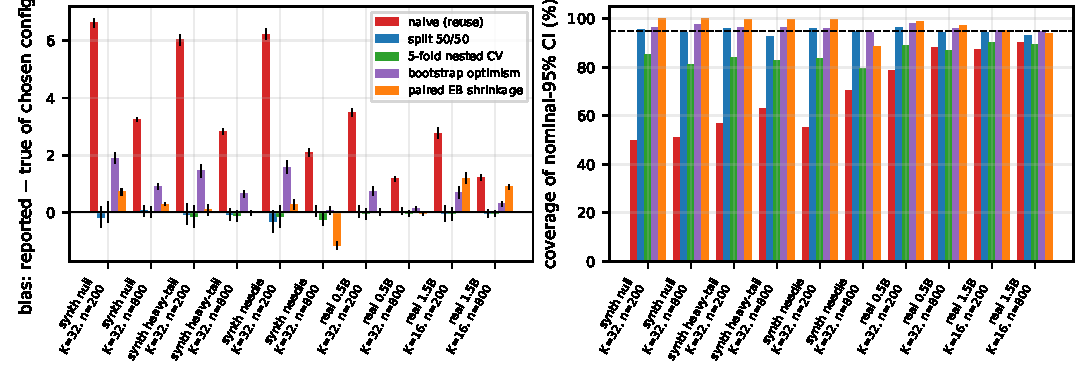
\includegraphics[width=\linewidth]{figs/fig_protocols.pdf}
\caption{Bias (left) and nominal-95\% interval coverage (right) of protocols across synthetic regimes and real LLMs (exhaustive search, $K=32$ or $K_{\rm tot}=16$). Error bars: 95\% CI over replicates. Dashed line: 95\%.}\label{fig:protocols}
\end{figure}
\begin{table}[h]
\caption{Select on STEM questions ($n$ per benchmark), deliver, evaluate on STEM and non-STEM (exhaustive). Gap = reported $-$ STEM-true, Shift = STEM-true $-$ non-STEM-true (pts, mean $\pm$ 95\% CI); Regret = best candidate's non-STEM accuracy $-$ delivered config's (pts).}\label{tab:shift}
\centering\footnotesize
\begin{tabular}{lrrrrrrrr}
\toprule Model & $K$ & $n$ & Reported & STEM & non-STEM & Gap & Shift & Regret\\ \midrule
0.5B & 4 & 100 & 17.2 & 14.5 & 17.4 & +2.71 $\pm$ 0.19 & -2.96 $\pm$ 0.07 & 1.04 \\
0.5B & 4 & 400 & 15.9 & 14.9 & 17.7 & +0.99 $\pm$ 0.10 & -2.74 $\pm$ 0.07 & 0.81 \\
0.5B & 16 & 100 & 19.4 & 14.9 & 17.7 & +4.54 $\pm$ 0.18 & -2.81 $\pm$ 0.07 & 1.92 \\
0.5B & 16 & 400 & 17.5 & 15.7 & 18.3 & +1.80 $\pm$ 0.10 & -2.58 $\pm$ 0.07 & 1.37 \\
0.5B & 32 & 100 & 20.3 & 15.0 & 17.7 & +5.28 $\pm$ 0.18 & -2.70 $\pm$ 0.07 & 2.19 \\
0.5B & 32 & 400 & 18.0 & 15.8 & 18.4 & +2.15 $\pm$ 0.10 & -2.56 $\pm$ 0.06 & 1.56 \\
1.5B & 4 & 100 & 27.7 & 25.6 & 33.1 & +2.14 $\pm$ 0.26 & -7.52 $\pm$ 0.09 & 0.67 \\
1.5B & 4 & 400 & 26.7 & 26.0 & 33.2 & +0.72 $\pm$ 0.13 & -7.18 $\pm$ 0.07 & 0.61 \\
1.5B & 16 & 100 & 30.1 & 26.0 & 33.1 & +4.15 $\pm$ 0.24 & -7.19 $\pm$ 0.08 & 1.21 \\
1.5B & 16 & 400 & 28.1 & 26.3 & 33.2 & +1.75 $\pm$ 0.12 & -6.88 $\pm$ 0.06 & 1.15 \\
\bottomrule
\end{tabular}
\end{table}
\begin{table}[h]
\caption{Full version of Table~\ref{tab:claims} (all $K$ and $n$).}\label{tab:claims_full}
\centering\footnotesize\setlength{\tabcolsep}{2.8pt}
\begin{tabular}{lrrrrrrrrrrrr}
\toprule & Base & & & Rep. & True & & \multicolumn{2}{c}{naive} & \multicolumn{2}{c}{split 50/50} & \multicolumn{2}{c}{max-$T$}\\
\cmidrule(lr){8-9}\cmidrule(lr){10-11}\cmidrule(lr){12-13}
Model & rank & $K$ & $n$ & impr. & impr. & $P_{\le0}$ & Claim & False & Claim & False & Claim & False\\ \midrule
0.5B & 1 & 4 & 200 & -0.38 & -2.19 & 100 & 2.6 & 2.6 & 2.7 & 2.7 & 0.9 & 0.9 \\
0.5B & 1 & 4 & 800 & -1.22 & -1.75 & 100 & 1.1 & 1.1 & 0.9 & 0.9 & 0.4 & 0.4 \\
0.5B & 1 & 16 & 200 & +1.25 & -1.63 & 100 & 6.8 & 6.8 & 2.2 & 2.2 & 0.1 & 0.1 \\
0.5B & 1 & 16 & 800 & +0.15 & -0.93 & 100 & 5.2 & 5.2 & 1.7 & 1.7 & 0.3 & 0.3 \\
0.5B & 1 & 31 & 200 & +1.95 & -1.50 & 100 & 12.2 & 12.2 & 2.6 & 2.6 & 0.3 & 0.3 \\
0.5B & 1 & 31 & 800 & +0.46 & -0.70 & 100 & 6.6 & 6.6 & 1.9 & 1.9 & 0.4 & 0.4 \\
0.5B & 4 & 4 & 200 & +0.14 & -1.64 & 83 & 4.4 & 2.8 & 2.4 & 1.7 & 1.2 & 0.7 \\
0.5B & 4 & 4 & 800 & -0.76 & -1.30 & 77 & 4.2 & 1.3 & 3.5 & 1.2 & 1.3 & 0.3 \\
0.5B & 4 & 16 & 200 & +1.80 & -1.07 & 72 & 11.2 & 6.9 & 3.0 & 0.9 & 1.0 & 0.5 \\
0.5B & 4 & 16 & 800 & +0.60 & -0.39 & 54 & 12.5 & 4.2 & 4.5 & 1.1 & 1.3 & 0.2 \\
0.5B & 4 & 31 & 200 & +2.43 & -0.98 & 68 & 17.6 & 11.0 & 3.6 & 0.9 & 1.2 & 0.4 \\
0.5B & 4 & 31 & 800 & +0.94 & -0.13 & 43 & 16.2 & 4.7 & 4.7 & 1.5 & 1.2 & 0.3 \\
1.5B & 1 & 4 & 200 & +0.42 & -0.95 & 100 & 4.4 & 4.4 & 3.4 & 3.4 & 1.0 & 1.0 \\
1.5B & 1 & 4 & 800 & -0.12 & -0.70 & 100 & 4.5 & 4.5 & 3.4 & 3.4 & 1.5 & 1.5 \\
1.5B & 1 & 15 & 200 & +2.13 & -0.74 & 100 & 14.9 & 14.9 & 3.9 & 3.9 & 1.6 & 1.6 \\
1.5B & 1 & 15 & 800 & +0.74 & -0.49 & 100 & 11.0 & 11.0 & 3.2 & 3.2 & 0.8 & 0.8 \\
1.5B & 4 & 4 & 200 & +0.92 & -0.53 & 76 & 7.9 & 5.5 & 4.4 & 3.0 & 3.0 & 1.6 \\
1.5B & 4 & 4 & 800 & +0.26 & -0.22 & 69 & 6.3 & 3.5 & 4.2 & 2.5 & 2.0 & 1.1 \\
1.5B & 4 & 15 & 200 & +2.34 & -0.27 & 66 & 16.2 & 10.1 & 2.9 & 2.3 & 2.0 & 1.4 \\
1.5B & 4 & 15 & 800 & +1.11 & +0.00 & 56 & 17.7 & 9.9 & 5.9 & 2.8 & 2.9 & 1.2 \\
\bottomrule
\end{tabular}
\end{table}

\begin{table}[h]
\caption{Two systems tuned on the same $n$-question benchmark with $K_A$ vs.\ $K_B$ random candidates. Rep./True gap: mean reported and true accuracy difference A$-$B (pts). $P_{\rm rep}$, $P_{\rm true}$: \% runs with reported / true gap $>0$. Claim: \% runs where a one-sided paired test (5\%) says A $>$ B; False: same, restricted to runs where A is truly not better. Naive = same benchmark for selection and test; split = select on half, test on other half.}\label{tab:systems}
\centering\footnotesize\setlength{\tabcolsep}{3pt}
\begin{tabular}{lrrrrrrrrrrr}
\toprule & & & & Rep. & True & & & \multicolumn{2}{c}{naive} & \multicolumn{2}{c}{split}\\
\cmidrule(lr){9-10}\cmidrule(lr){11-12}
Model & $K_A$ & $K_B$ & $n$ & gap & gap & $P_{\rm rep}$ & $P_{\rm true}$ & Claim & False & Claim & False\\ \midrule
0.5B & 16 & 2 & 100 & +4.00 & +0.74 & 87 & 63 & 16.8 & 11.7 & 8.0 & 3.8 \\
0.5B & 16 & 2 & 400 & +2.38 & +1.27 & 87 & 76 & 30.4 & 7.6 & 15.9 & 3.0 \\
0.5B & 16 & 2 & 800 & +2.20 & +1.62 & 88 & 81 & 46.9 & 3.7 & 21.4 & 1.3 \\
0.5B & 8 & 2 & 100 & +2.62 & +0.59 & 73 & 62 & 9.9 & 3.7 & 7.7 & 3.8 \\
0.5B & 8 & 2 & 400 & +1.81 & +1.04 & 77 & 69 & 23.4 & 3.6 & 13.2 & 1.8 \\
0.5B & 8 & 2 & 800 & +1.53 & +1.10 & 78 & 71 & 34.4 & 4.8 & 20.7 & 0.9 \\
0.5B & 2 & 2 & 100 & -0.03 & -0.02 & 46 & 47 & 3.8 & 1.3 & 6.8 & 2.0 \\
0.5B & 2 & 2 & 400 & +0.11 & +0.13 & 50 & 52 & 9.9 & 1.0 & 9.4 & 1.7 \\
0.5B & 2 & 2 & 800 & +0.06 & +0.05 & 50 & 51 & 15.6 & 1.0 & 14.3 & 2.0 \\
1.5B & 8 & 2 & 100 & +2.79 & +0.54 & 77 & 57 & 14.5 & 7.9 & 9.6 & 5.1 \\
1.5B & 8 & 2 & 400 & +1.57 & +0.65 & 78 & 63 & 20.9 & 7.9 & 11.2 & 4.1 \\
1.5B & 8 & 2 & 800 & +1.29 & +0.63 & 78 & 64 & 26.4 & 5.2 & 14.3 & 2.6 \\
1.5B & 2 & 2 & 100 & +0.02 & +0.04 & 45 & 49 & 5.3 & 2.7 & 8.2 & 4.3 \\
1.5B & 2 & 2 & 400 & +0.02 & +0.00 & 47 & 47 & 10.7 & 2.1 & 8.6 & 2.1 \\
1.5B & 2 & 2 & 800 & -0.03 & -0.01 & 48 & 48 & 15.6 & 1.9 & 11.7 & 2.5 \\
\bottomrule
\end{tabular}
\end{table}

\begin{table}[h]
\caption{Protocols in the synthetic ``spread'' regime (configuration effects $\mathcal N(0,3\text{ pts}^2)$, $K{=}32$, $n{=}200$); columns as in Table~\ref{tab:protocols}.}\label{tab:protocols_spread}
\centering\footnotesize
\begin{tabular}{llrrrr}
\toprule Setting & Protocol & Bias & RMSE & Cov & Width\\ \midrule
synth spread & naive (reuse) & +5.30 $\pm$ 0.20 & 5.84 & 74 & 13.6 \\
synth spread & split 20/80 (sel/rep) & -0.14 $\pm$ 0.64 & 7.93 & 94 & 28.4 \\
synth spread & split 50/50 & +0.04 $\pm$ 0.38 & 4.75 & 95 & 18.5 \\
synth spread & 5-fold nested CV & -0.35 $\pm$ 0.39 & 4.87 & 82 & 13.2 \\
synth spread & bootstrap optimism & +1.10 $\pm$ 0.24 & 3.15 & 96 & 13.7 \\
synth spread & paired EB shrinkage & +0.18 $\pm$ 0.20 & 2.49 & 99 & 13.7 \\
synth spread & max-$T$ simultaneous CI & -- & -- & 98 & 21.8 \\
\bottomrule
\end{tabular}
\end{table}

\subsection{Pool truth vs.\ out-of-sample truth}\label{app:oos}
The pool is finite, so the benchmark sample $S$ overlaps the pool-mean truth. Re-measuring the same replicates against the accuracy of the delivered configuration on the pool questions \emph{not} in $S$ (without-replacement analogue; it is anti-correlated with the in-sample accuracy by construction and hence biased upwards in gap) gives the following; the pool-truth gap of the main text is the exact i.i.d.\ quantity, this table is the upper end of the bracket.
\begin{table}[h]
\caption{Gap (pts) of naive and bootstrap-corrected reports against pool truth and against out-of-sample truth ($K=K_{\rm tot}$, exhaustive).}\label{tab:oos}
\centering\footnotesize
\begin{tabular}{lrrrrr}
\toprule Model & $n$ & naive (pool) & naive (oos) & boot.\ opt.\ (pool) & boot.\ opt.\ (oos)\\ \midrule
0.5B & 100 & +5.36 & +5.71 & +1.19 & +1.54 \\
0.5B & 400 & +2.07 & +2.60 & +0.33 & +0.87 \\
0.5B & 800 & +1.17 & +1.81 & +0.14 & +0.78 \\
1.5B & 100 & +4.02 & +4.43 & +0.99 & +1.40 \\
1.5B & 400 & +1.83 & +2.59 & +0.44 & +1.19 \\
1.5B & 800 & +1.22 & +2.23 & +0.30 & +1.31 \\
\bottomrule
\end{tabular}
\end{table}

\section{Reproducibility}\label{app:repro}
\paragraph{Environment.} Python 3.11, torch 2.15.0+cpu, transformers 5.22.2, numpy 2.4.6, scipy 1.17.1, pandas 3.0.6, pyarrow 26.0.1, matplotlib 3.11.2; Intel Xeon Gold 6230 (40 logical cores shared with other jobs, 251 GB RAM), no GPU. Data: \texttt{TIGER-Lab/MMLU-Pro} revision \texttt{b189ec765aa7ed75c8acfea42df31fdae71f97be} (MIT licence); models \texttt{Qwen/Qwen2.5-\{0.5,1.5\}B-Instruct} (Apache-2.0 for 0.5B and 1.5B), fp32. Seeds: pool/config seed 0; simulation seeds are in the scripts (\texttt{--seed}).
\paragraph{Compute actually used.} LLM scoring (4 threads per job, CPU contention from other tenants; wall-clock): 7.3 h (0.5B, $32\times1500$), 5.8 h (1.5B, $16\times1000$), plus the fresh-question matrices (\S\ref{sec:fresh}; run concurrently: 7.8 h for $32\times1000$ and 7.5 h for $16\times600$), i.e.\ 28.4 job wall-hours in total (\texttt{results/compute\_usage.txt}); statistical simulations: about 0.3 CPU-hours per real-data experiment and a few CPU-hours for the synthetic study. Preliminary runs not in the paper: speed/accuracy checks on 96 questions (including torch int8 dynamic quantisation, which we abandoned because it halved accuracy), and a first synthetic run (superseded after adding the needle-size sweep and $\mu$-spread diagnostics; no results were dropped). No hyperparameter of any protocol was tuned on the reported results.
\paragraph{Scripts $\to$ outputs.} See \texttt{README.md} in the code package for commands and expected runtimes.
\begin{center}\footnotesize\begin{tabular}{ll}
\toprule Output & Script\\ \midrule
correctness matrices & \texttt{code/get\_data.py}, \texttt{code/run\_scoring.sh}, \texttt{code/run\_fresh*.sh} ($\to$ \texttt{score.py}, \texttt{prompts.py})\\
Fig.~\ref{fig:scaling}, Tab.~\ref{tab:curse},\ref{tab:gain},\ref{tab:curse_full} & \texttt{exp\_real.py}, \texttt{exp\_synth.py}, \texttt{make\_report.py}\\
Tab.~\ref{tab:claims}--\ref{tab:shift} & \texttt{exp\_decisions.py}, \texttt{make\_report.py}\\
Tab.~\ref{tab:protocols}, Fig.~\ref{fig:protocols}, Tab.~\ref{tab:synth_scale}--\ref{tab:lower} & \texttt{exp\_real.py}, \texttt{exp\_synth.py}, \texttt{make\_report.py}\\
Fig.~\ref{fig:split} & \texttt{exp\_split.py}, \texttt{make\_report.py}\\
Sec.~\ref{sec:fresh} & \texttt{exp\_fresh.py}, \texttt{make\_report.py}\\
Tab.~\ref{tab:oos} & \texttt{exp\_real.py} (oos fields), \texttt{make\_report.py}\\
matrix statistics (\S\ref{sec:setup}) & \texttt{describe\_matrix.py}\\
\bottomrule\end{tabular}\end{center}
\paragraph{Literature handling.} Only the starter references and a few classical model-selection references were consulted (titles/authors checked via Crossref/arXiv metadata, \texttt{code/check\_refs.py}); no material excluded by the task statement was searched for, opened or read, and none was encountered.
